
\documentclass{article}
\usepackage[left=2.5cm,top=2.5cm,right=2.5cm,bottom=2.5cm]{geometry}
\usepackage{amsmath}
\usepackage{array}
\usepackage{caption}
\usepackage{placeins}
\usepackage{graphicx}
\usepackage{subcaption}
\usepackage{setspace}
%\usepackage[active,tightpage]{preview}
\usepackage{natbib}
\bibpunct{(}{)}{,}{a}{}{;} 
\usepackage{url}
\usepackage{nth}
\usepackage{authblk}
\usepackage{listings}
% for the d in integrals
\newcommand{\dd}{\; \mathrm{d}}
\newcommand{\tc}{\quad\quad\text{,}}
\newcommand{\tp}{\quad\quad\text{.}}
\bibliographystyle{apalike}

\title{The Contributions of Homicides an Other Health Interventions to the  Best Practices Life Expectancy in Mexico, 1990-2010}

\author[1]{Jose Manuel Aburto\thanks{aburtoflores@demogr.mpg.de}}
\author[2]{Tim Riffe}
\affil[1]{Max Planck Institute for Demographic Research, EDSD}
\affil[2]{Max Planck Institute for Demographic Research}


\begin{document}

\maketitle

\begin{abstract}
Progress in life expectancy in Mexico has


\end{abstract}


\section*{Background}
The \nth{20} century was marked by sizable improvements in mortality, living
conditions and health in most Latin American countries \citep{who2000}. In
Mexico, these improvements have slowed down recently as a result of opposing
trends in particular causes of death. For instance, homicide and diabetes
increased drammatically, even as infectious and
respiratory diseases continued to fall. While life
expectancy at birth increased by 4.3 years for males (from 67.6 to 71.9) and 3.4
for females (from 73.8 to 77.2) between 1990 and 2000 \citep{SOMEDE},
between 2000 and 2010, life expectancy at birth entered into a period of
stagnation for males and slowed progress for females \citep{canudas2014}. This
period coincides with the implementation of different public health
interventions, such as the Universal Vaccination Program and Seguro
Popular, which aim to provide primary and secondary
health care to the uninsured population, allocate funds to cover catastrophic
health expenditures \citep{knaul2005}. Further, the Oportunidades program
was introduced to supply incentives for families to invest in themselves and
benefit from education, health, and nutrition \citep{neufeld2012}. Some evidence
suggests that Mexico experienced substantial decreases in infant and child
mortality, along with improvements that contributed to the reduction of
mortality and in the prevalence of acute malnutrition between 1980 and 2000
because of these interventions \citep{sepulveda2006}. Similarly, some evidence
suggests that by 2012 Seguro Popular had covered an additional 52 million
people in Mexico that did not have any access to public health care and, as a result, there has been a reduction in catastrophic health expenditures \citep{knaul2012}.

 Although these results are important, they do not reveal heterogeneity between
 Mexican states, which is an important task given the high degree of social and
 health inequalities in Mexico \citep{Frenk2006}. Given these improvements
 in health care coverage, the strong role of institutions, and ongoing public
 health interventions, it is necessary to assess the varied impacts that
 these health interventions may have had on particular causes of death in states
 populations and across the country.
 
 One approach to assess the impact of health services is by operationalizing the
 concept of Avoidable/Amenable Mortality (hereafter abbreviated AM)
 \citep{nolte&mckee2004, nolte&mckee2008}. This construct aims to measure the quality of health service systems by selecting certain
 causes of death that should not occur in the presence of effective and
 timely health care. Among industrialized countries (e.g., United States,
 Australia, France, Japan), a reduction in AM rates was
 observed from the late 1990's into the \nth{21} Century
 \citep{nolte&mckee2008}. Avoidable mortality rates fell, on average, by 17\%
 for males and 14\% for females in these countries. Despite mortality reductions for
 both sexes, heterogeneity between countries was identified, with the United
 States showing the smallest reductions (around 5\%) for both sexes. However,
 each country showed progress in mortality from treatable cancers and
 circulatory diseases except for ischemic heart diseases.

In Mexico, the components of avoidable mortality had different trends since the
late 1990's. Between 2000 and 2004 AM decreased, particularly from
infectious diseases and nutrition-related conditions \citep{francomarina2006}, while it increased between 1998 and 2010 due to diabetes, circulatory diseases, perinatal and respiratory conditions
\citep{agudelo2014efecto}. Increases in the latter causes
of death were particularly concentrated in the poorest states of the country
\citep{davila2014mortalidad}. We aim to improve on these studies
by a more focused segmentation of AM into health intervention-related AM and
behavior-related AM. Also, we extend analysis to all 32 states, by sex, and over
the full 21-year period from 1990 to 2010.\footnote{In the final revision of
this paper we will provide series through 2013. Right now the exposures are not
yet prepared for years after 2010.} Finally, we compare state mortality patterns
with best-practice benchmarks for large age groups. These best practice
benchmarks are calculated on the basis of the lowest observed mortality within
ages and causes, among the full set of 32 Mexican states. This concept was first
proposed by \citet{wunsch1975minimum}, later explored by
\citet{vallin2008minimum}, and more recently applied under a different
definition by \citet{eikemo2014}. We apply standard decomposition techniques to
isolate the cause and age-specific shortcomings between states and the
corresponding best-practices lifetable. 

\section*{Data \& Methods} 
 
We used death counts available from official microdata files produced by the
Mexican Statistical Office from 1990 to 2010 \citep{INEGI}. These data contain
information on causes of death by single age, sex, and place of residence at the
time of death. In addition, we used population estimates (Exposures) corrected
for age misstatement, undercounting, and migration--- both internal and
international--- available from the \citet{SOMEDE} to construct
cause-age-specific death rates by sex and state from 1990 to 2010.

\subsection*{Classification of Causes of Death}

To separate causes of death that are susceptible to medical intervention (e.g.,
infectious and respiratory diseases) and those related to health behaviors and
intersectoral policies (e.g., homicides, lung cancer) we use the concept of
'Amenable/Avoidable Mortality' (AM) (cite Nolte and Mackee 2004,2008). This
concept assumes a list of conditions that should not occur with the availability
of timely medical care. Recently, this concept has also been used to gauge the
effect of causes that can be influenced by public policy (e.g., cirrhosis)(cite
Elo 2014). We classified causes of death into ten groups based on prior studies
(cite Elo 2014)(cite aburto 2015), as listed in Table~\ref{tab:causes}, with
relative frequencies by sex.

% latex table generated in R 3.1.2 by xtable 1.7-4 package
% Wed Sep 23 21:57:18 2015
\begin{table}[ht]
\centering
\caption{Ten major cause groups, with crude percentages below age 75.}
\label{tab:causes}
\begin{tabular}{>{\raggedright}m{3cm}rr}
 Cause & Males & Females \\ 
  \hline
causes amenable to medical service & 28.50 & 40.24 \\ 
  diabetes & 9.07 & 14.77 \\ 
  ischemic heart diseases & 7.92 & 6.66 \\ 
  HIV/AIDS & 1.80 & 0.51 \\ 
  lung cancer & 1.58 & 1.09 \\ 
  cirrhosis & 5.34 & 1.09 \\ 
  homicide & 5.95 & 1.05 \\ 
  road traffic accidents & 5.82 & 2.26 \\ 
  suicide & 1.48 & 0.46 \\ 
  other causes & 32.53 & 31.86 \\ 
   \hline
\end{tabular}
\end{table}

We separate diabetes, ischemic heart diseases (IHD), HIV/AIDS, lung
cancer, and cirrhosis because all of them are amenable to both health behavior
and medical service, and because the first two represent major causes of death
in Mexico \citep{canudas2014}. In addition to these causes, we also isolate
homicide, road traffic accidents, and suicide because they have emerged as
leading causes of death among young people, and the first two had a sizeable
impact on life expectancy recently in Mexico \citep{canudas2014}. All causes of death were classified using the International Classification of Diseases, revision 9 for the period 1990-1997 and the tenth revision for 1998-2010 (see Apppendix Table 1 for details on ICD codes for each cause).

We truncated analysis at age 75 because classification of causes of deaths and age reporting are considered to be innacurate in death registration at older ages (cite Tobias \& Jackson 2001) and because most changes in life expectancy are likely due to changes in mortality patterns below the age of 75 (cite Aburto 2015). In addition, health care and policy/behavior interventions are more likely to be effective at younger ages (cite Elo 2014).


\subsection*{Demographic Methods}
We first calculated age-sex-cause specific death rates for the 32 states up to age 75 and estimated period life tables for females and males from 1990 to 2010 following standard life table techniques (cite preston 2001). Second, we estimated temporal life expectancy to capture differential effects of the morality categories among three subgroups: child (ages 0-14), young (ages 15-40) and adult (40-75). We did this following procedures previously used (Arriaga 1984). 

We then constructed the Best Practices Lifetable (BP) for every year and estimated cause-specific contributions to the difference between state-specific temporary life expectancy and BP temporary life expectancy ($e^{\star}$) applying standard decomposition methods (cite horiuchi wilmoth). All the analyses 


\subsection*{Best Practices Lifetable}
This approach was first proposed by cite(Vallin \& Mesle (2008)), and we summarize it
briefly here. The imaginary BP lifetable is a composite
of the lowest observed mortality rates by age, cause, and state for a given sex
and year. In continous terms, we define life expecancy, $e(0)$, as:
\begin{equation}
\int _0 ^\infty l(x) \dd x \tc
\end{equation}
where $l(x)$ is the survivorship function defined with radix of one, or as a
function of the force of mortality, $\mu(x)$ as:
\begin{equation}
\label{eq:lx}
l(x) = e^{-\int_0^x \mu(a) \dd a}
\end{equation}

In general, $\mu(x)$ can be treated as the sum of $I$ cause-specific mortality
rates at age $x$ assuming that causes of death are independent of one another like $\mu(x) = \sum_1^I \mu_i(x)$. In the case of best practices mortality we treat $\mu(x)$ as a composite of the lowest observed cause-specific mortality rates in the given age $x$.

\begin{equation}
\label{eq:mxmin}
\mu(x)^{\star} = \sum_1^I min(\mu_i(x))
\end{equation}

This BP $\mu^{\star}(x)$ has a unique age profile, and it uniquely
determines a pattern of $l(x)^{\star}$, per \eqref{eq:lx}, that corresponds with a
best practices life expectancy, $e(0)^{\star}$. Thus, $e(0)^{\star}$ can be treated as a
maximum presently acheivable life expectancy given the best available
practices and technologies within a given set of populations and assuming
perfect diffussion (cite Vallin \& Mesle). It is an imaginary quantity because no particular population
ever acheives this mortality pattern, and none may ever. However, this value is
a real referent not based on a projection of improvements into the future, and
so it bounds our optimism in a practical way.

\subsection*{Temporary Life Expectancy}

We require an estimate of temporary life expectancy between ages
$x_1$ and $x_2$, for $x_1<x_2$, or the average years of life lived between these ages according to a given set of period mortality rates (cite arriaga 1984). We denote this quantity as
$e(x_1,x_2)$, and its best practices maximum as $e^{\star}(x_1,x_2)$. Defined in
terms of $l(x)^\star$:


\begin{equation}
e^{\star}(x_1,x_2) = \frac{\int _{x_1}^{x_2} l(x)^\star \dd x}{l(x_1)^\star}
\end{equation}

\subsection*{Cause Specific Contributions to the difference between
$e_x^{\star}(x_1,x_2)$ and $e_x(x_1,x_2)$}

To estimate the contributions of every category of avoidable mortality to the difference between BP temporary life expectancy and regular temporary life expectancy we use the line integral model (Horiuchi etal 2008). Let $\Delta$ represent the gap between $e_x^{\star}(x_1,x_2)$ and $e_x(x_1,x_2)$. In descrete formulation


\subsection*{Limitations}
The limitations of our study should be mentioned. First, mortality data are likely to present innacuracies in cause-of-death classification, particularly at older ages (cite Tobias and Jackson). To mitigate this, we focus on ages below 75 grouping causes of death according to the 'avoidable mortality' concept using ICD codes. Second, our estimates regarding homicide mortality are likely to be underestimated because of inaccurate practices regarding counting, reporting and because the large number of missing individuals in Mexico (cite HRW). Third, the 'Avoidable Mortality' concept should be understood as an indicator of potential weaknesses with respect to health care and some public health policies and not as a definitive assessment. Fourth, the amount of deaths that should be considered avoidable within the avoidable classification is not clear in the literature (cite beltran-sanchez chapter); we overcame this by applying a methodological framework based on mortality levels that had been observed and therefore pontentially achievable within the states.

Despite these limitations, we made use of the most reliable data available publicly to perform our analyses in a 20-year period at the subnational level in Mexico accounting for all the categories we were interested.



\section*{Results}
\subsection{Trends in best practices life expectancy}


\begin{figure}
\centering
\caption{Temporary life expectancy for states (black line), vanguard life
expectancy (red) and best practices life expectancy  $e^\star (0,14)$ (blue) by
sex, 1990-2010.}
\begin{subfigure}{\textwidth}
\centering
\caption{$e(0,14)$}
\label{fig:e0_14}
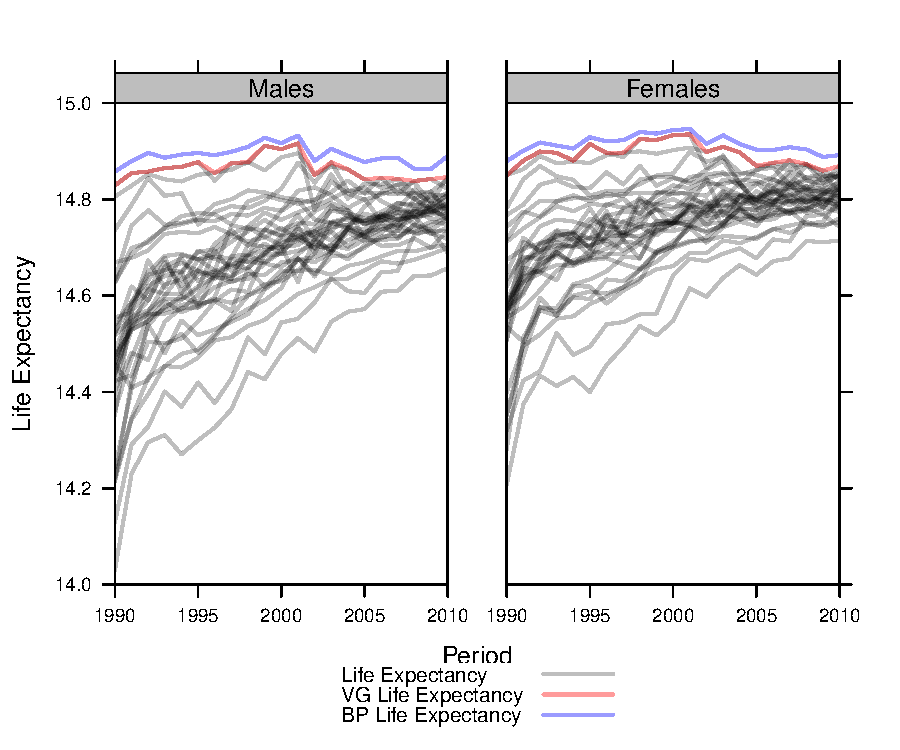
\includegraphics[scale=.5]{Figures/et0_14.pdf}
\end{subfigure}
\\
\begin{subfigure}{\textwidth}
\centering
\caption{$e(15,39)$}
\label{fig:e15_39}
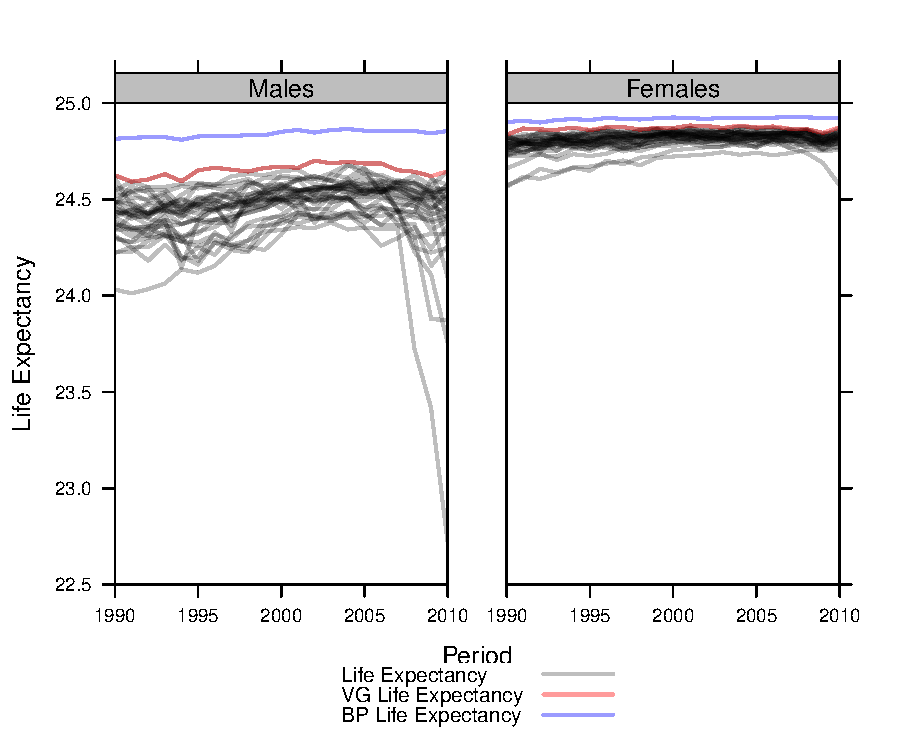
\includegraphics[scale=.5]{Figures/et15_39.pdf}
\end{subfigure}
\\
\begin{subfigure}{\textwidth}
\centering
\caption{$e(40,74)$}
\label{fig:e40_74}
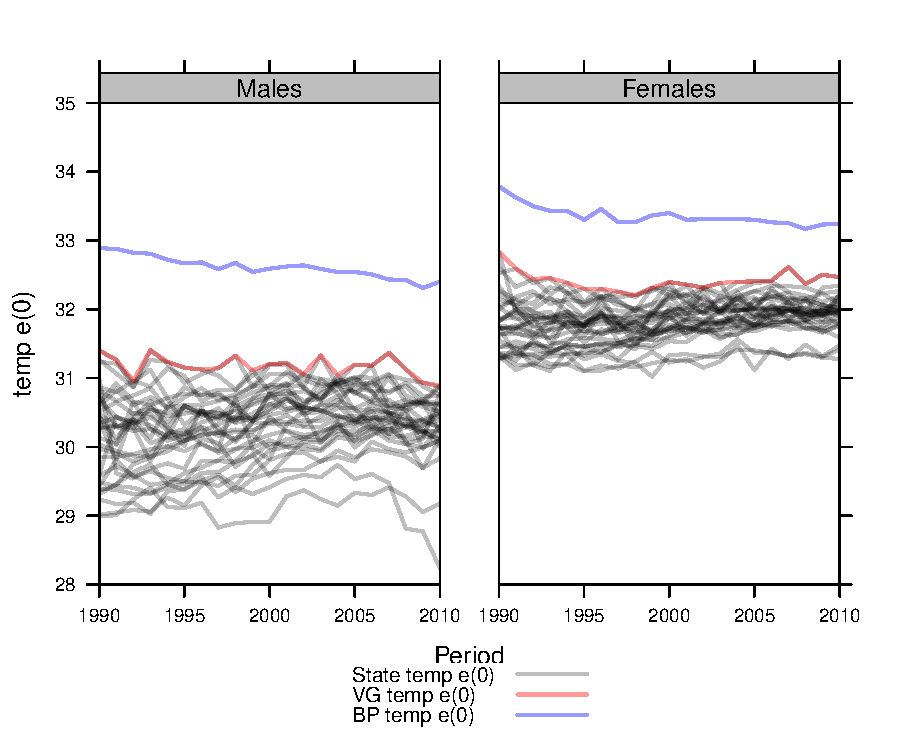
\includegraphics[scale=.5]{Figures/et40_74.pdf}
\end{subfigure}
Source: own calculations based on INEGI and SOMEDE files. 
\end{figure}


\subsection*{State trends in departures from best practices temp e(0)}
Small multiples maps (time series of maps)

\subsection*{Age and cause contributions to differences}

This will show a few small multiples figures, tbd 

\section*{Discussion}
Talk about the role of homicide and other major causes. How many years of life
were lost? (not just expectancy). maybe..

\section*{Conclusions}
Homicide is a public health concern..


%}
%\bibliographystyle{plainnat}
 \bibliography{AburtoRiffe_Bib.bib}

\end{document}


